\chapter{Advanced Algorithms}
\label{chap:advanced_algorithms}

\begin{figure}[ht]
	\hfill
	\begin{minipage}{0.5\textwidth}
		\centering
		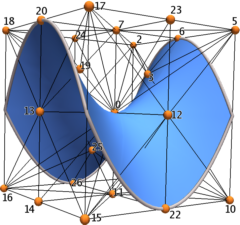
\includegraphics{VTKTextbook-168}
		\caption*{\texttt{An isocontour of a tri-quadratic Lagrange-interpolant. Image courtesy D. Thompson and P. Pébay Sandia National Labs.}}
	\end{minipage}
\end{figure}

\firstletter{W}e return again to visualization algorithms.
This chapter describes algorithms that are either more complex to implement, or less widely used for 3D visualization applications.
We retain the classification of algorithms as either scalar, vector, tensor, or modelling algorithms.

\section{Scalar Algorithms}

As we have seen, scalar algorithms often involve mapping scalar values through a lookup table, or creating contour lines or surfaces.
In this section, we examine another contouring algorithm, dividing cubes , which generates contour surfaces using dense point clouds.
We also describe carpet plots.
Carpet plots are not true 3D visualization techniques, but are widely used to visualize many types of scalar data.
Finally, clipping is another important algorithm related to contouring, where cells are cut into pieces as a function of scalar value.

\subsection{Dividing Cubes}

\section{Vector Algorithms}

\subsection{Vector Field Topology}

\begin{figure}[htb]
	\begin{subfigure}[h]{0.32\linewidth}
		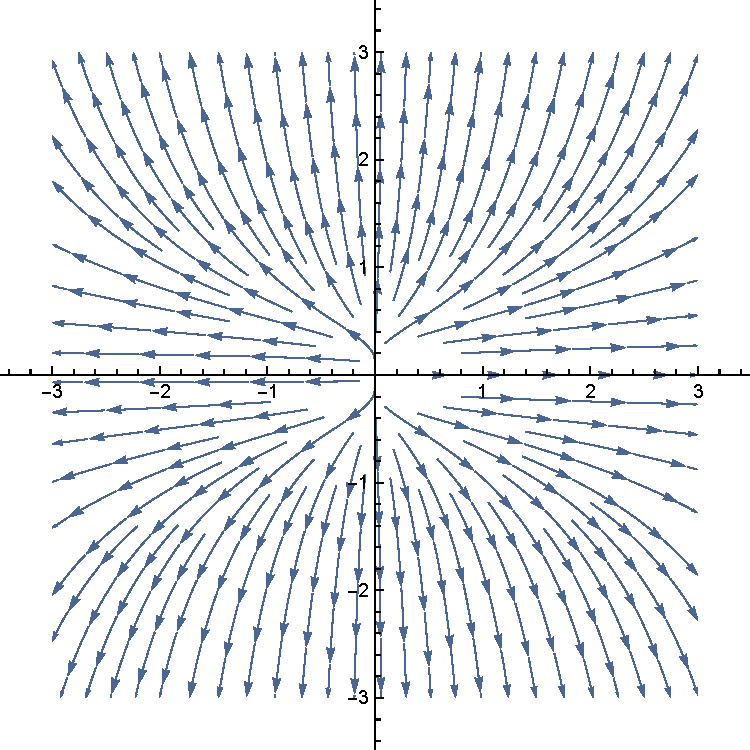
\includegraphics[width=0.86\linewidth]{Figure9-13a}
		\captionsetup{justification=centering}
		\caption*{Repelling Node\\$R_1, R_2 > 0$\\$I_1, I_2 = 0$}
		\label{fig:Figure9-13a}
	\end{subfigure}
	\hfill
	\begin{subfigure}[h]{0.32\linewidth}
		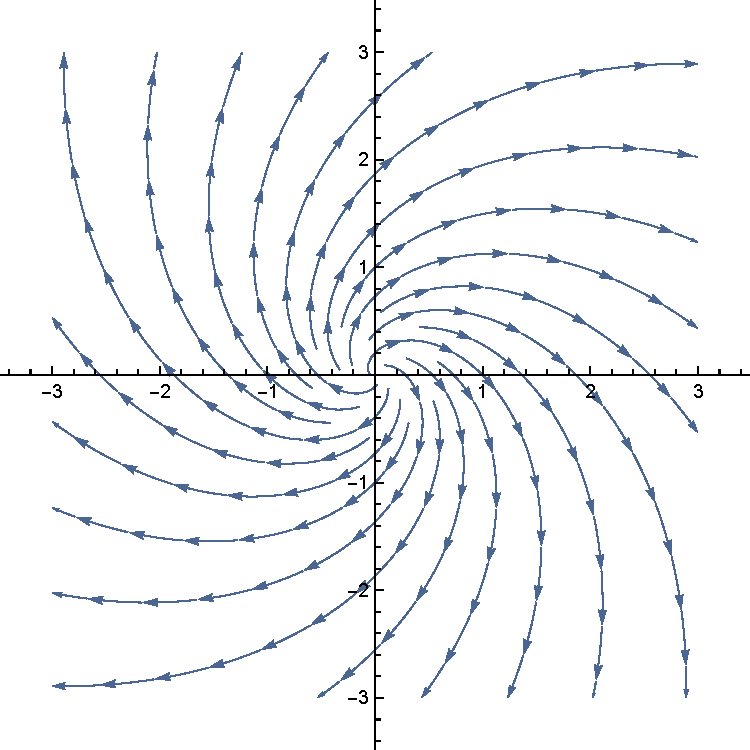
\includegraphics[width=0.86\linewidth]{Figure9-13b}
		\captionsetup{justification=centering}
		\caption*{Repelling Focus\\$R_1, R_2 > 0$\\$I_1, I_2 \neq 0$}
		\label{fig:Figure9-13b}
	\end{subfigure}
	\hfill
	\begin{subfigure}[h]{0.32\linewidth}
		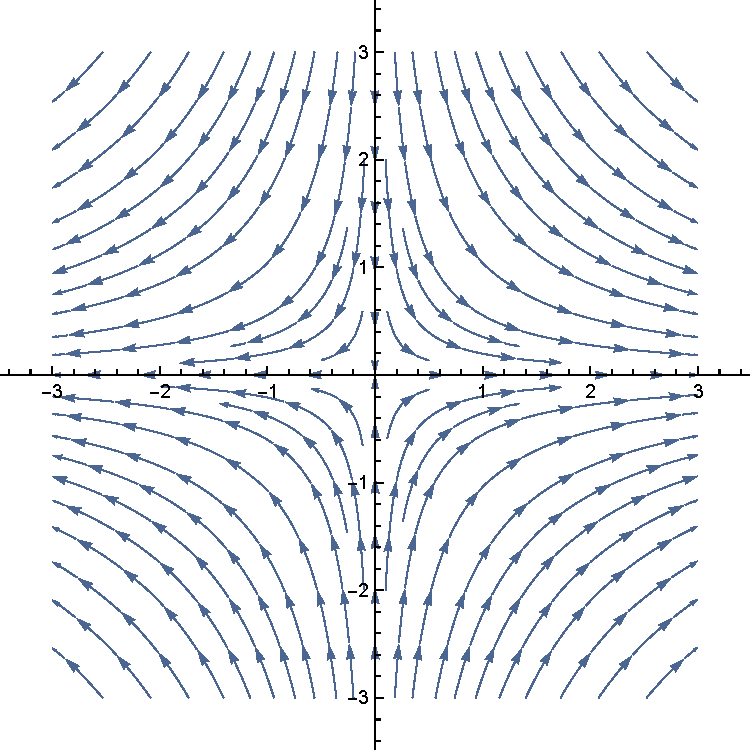
\includegraphics[width=0.86\linewidth]{Figure9-13c}
		\captionsetup{justification=centering}
		\caption*{Saddle Point\\$R_1 \times R_2 < 0$\\$I_1, I_2 = 0$}
		\label{fig:Figure9-13c}
	\end{subfigure}
	\hfill
		\begin{subfigure}[h]{0.32\linewidth}
		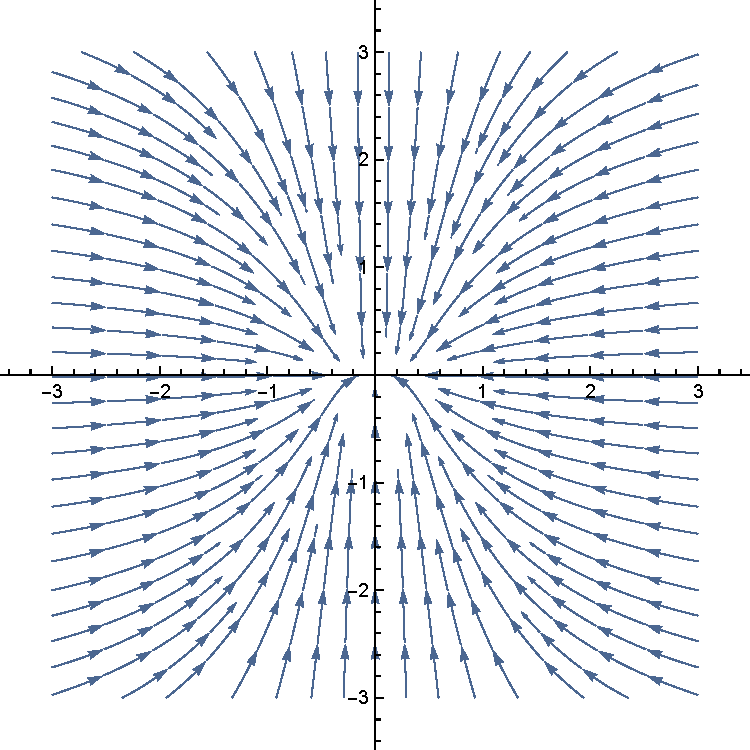
\includegraphics[width=0.86\linewidth]{Figure9-13d}
		\captionsetup{justification=centering}
		\caption*{Attracting Node\\$R_1, R_2 < 0$\\$I_1, I_2 = 0$}
		\label{fig:Figure9-13d}
	\end{subfigure}
	\hfill
	\begin{subfigure}[h]{0.32\linewidth}
		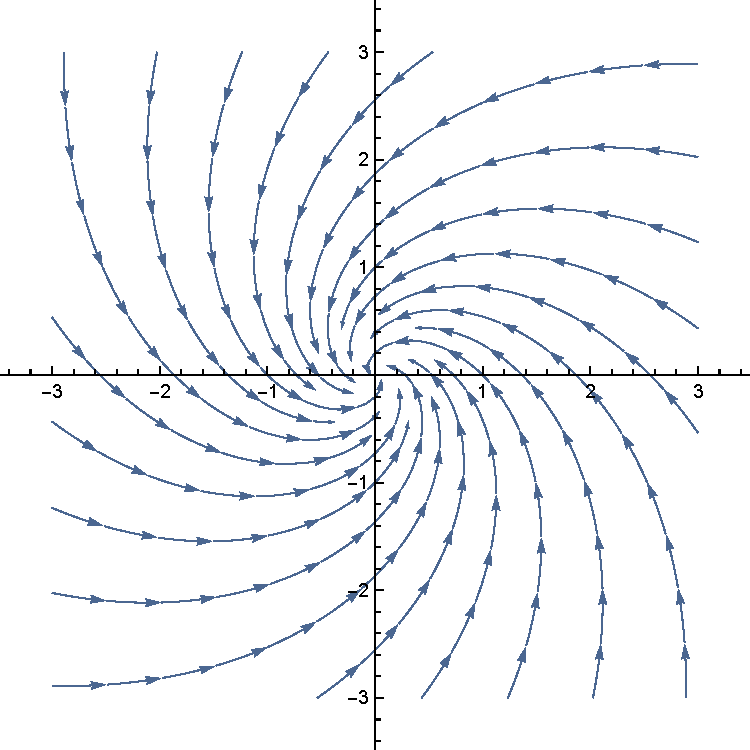
\includegraphics[width=0.86\linewidth]{Figure9-13e}
		\captionsetup{justification=centering}
		\caption*{Attracting Focus\\$R_1, R_2 < 0$\\$I_1, I_2 \neq 0$}
		\label{fig:Figure9-13e}
	\end{subfigure}
	\hfill
	\begin{subfigure}[h]{0.32\linewidth}
		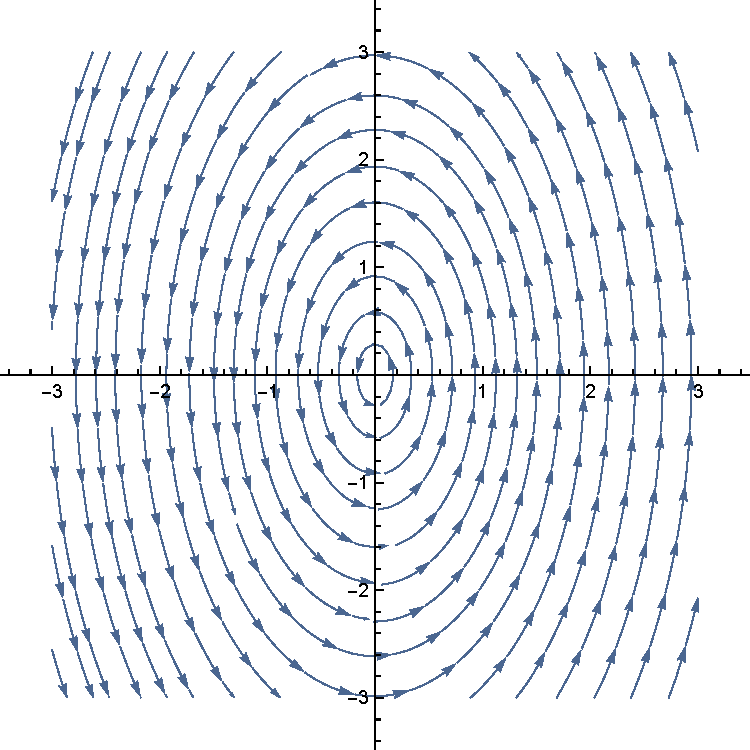
\includegraphics[width=0.86\linewidth]{Figure9-13f}
		\captionsetup{justification=centering}
		\caption*{Center\\$R_1, R_2 = 0$\\$I_1, I_2 \neq 0$}
		\label{fig:Figure9-13f}
	\end{subfigure}
	\caption{Critical points in two dimensions. The real part of the eigenvalues ($R_1$, $R_2$) of the matrix of first derivatives control the attraction or repulsion of the vector field. The imaginary part of the eigenvalues ($I_1$, $I_2$) controls the rotation.}\label{fig:Figure9-13}
\end{figure}


\begin{equation}\label{eq:9.12}
H_d = \overrightarrow{v\ } \cdot \overrightarrow{w\ } = \vert \overrightarrow{v\ } \vert \vert \overrightarrow{w\ } \vert \cos(\phi)
\end{equation}
\myequations{Scalar function of the vector dot product. }

\section{Tensor Algorithms}

\section{Modelling Algorithms}

\subsection{Mesh Smoothing}
\label{subsec:mesh_smoothing}

\subsection{Visualizing Unstructured Points}
\label{subsec:visualizing_unstructured_points}

\subsection{Texture Algorithms}
\label{subsec:texture_algorithms}

\section{Putting It All Together}

\subsection{Connectivity}
\label{subsec:connectivity}